It is the user interface (UI) that the user interacts with. The interface itself, as
shown in \autoref{fig:figure1}, is broken down into a number of separate areas:

\begin{figure}[!htbp]
  \centering {
    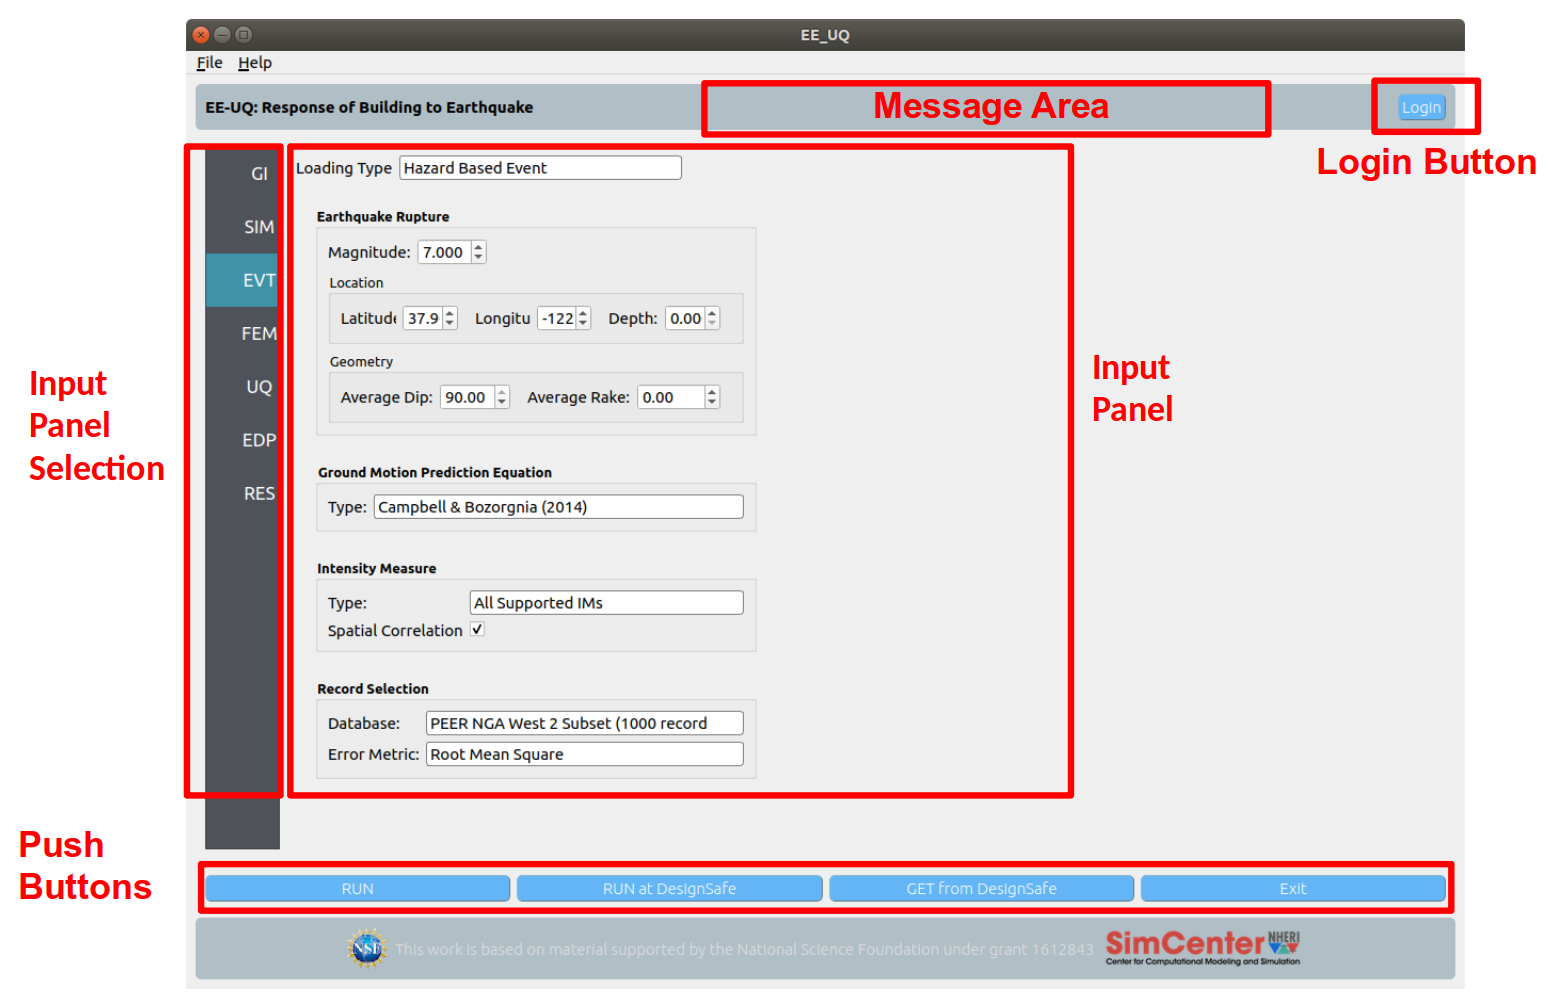
\includegraphics[width=0.8\textwidth]
    {usage/figures/ui.png} }
  \caption{UI}
  \label{fig:figure1}
\end{figure}

\begin{enumerate}
\item Input Panel Selection: This area on the left side provides the
  user with a selection of items to choose from from:
\begin{enumerate}
  \item GI: General information, for specifiction of building
    description, location and units.
  \item SIM: Structure information model, for description of the
    building model.
  \item EVT: Event, for selecting the earthquake motions input.
  \item FEM: Finite element method, for specification of application
    and analysis options.
  \item UQ: Uncertainty quantification, for defining the distribution
    of the random variable paramaters and UQ method analysis options.
  \item EDP: Engineering demand parameters, for specification of
    output response quantities.
  \item RES: Results output.
\end{enumerate}

Selecting any of these will change the input panel presented.

\item Input Panel: This is the large central area of the UI that the
  user provides input for the application chosen and views the
  results. For example if the user had selected UQ in the input panel
  selection, it is in this panel that the user would provide details
  on the distributions associated with each random variable or select
  the sampling method to use and provide the options necessary to run
  that method.

\item Push Buttons: This is the area near the bottom of the UI in
  which 4 buttons are presented to the user:

\begin{enumerate}
\item RUN – to run the simulation of the user’s desktop machine.
\item RUN at DesignSafe – to process the information, and send to
  DesignSafe where the job will be run on a supercomputer and results
  stored in your DesignSafe jobs folder.
\item GET from DesignSafe – to obtain from DesignSafe your list of
  jobs and select from that list a job to download.
\item Exit: to exit the application.
\end{enumerate}

The Screens presented to user when the first 3 of these buttons will
be discussed in section 3.10.

\item Login Button: At the top right of the UI is the login
  button. Before the user can launch any jobs on DesignSafe they must
  first login to DesignSafe using their DesignSafe login and
  password. Pressing the login button will open up the login window
  for users to enter this information.

\item Message Area: In the top center of the application is the area
  of the interface that error and status messaged will be displayed
  while the application is running.

\end{enumerate}
